\chapter{Platform Operations}

\chapterquote{The best investment on earth is earth.}{Louis Glickman}

\section*{Introduction}
\addcontentsline{toc}{section}{Introduction}

This chapter presents the core investment features that complement the AI capabilities and blockchain infrastructure of the Korpor platform. These features focus on enhancing the investor experience through comprehensive property management and portfolio tracking. The implementation covers property listing management and investment portfolio analytics for both web and mobile interfaces.

\section{Sprint 8: Property Management \& Investor Portfolio}

\subsection*{Introduction}
The Property Management \& Investor Portfolio sprint focuses on establishing comprehensive property listing management functionality and providing detailed investment tracking capabilities. This foundation enables real estate agents and administrators to efficiently manage property portfolios while allowing investors to monitor their investments and analyze their real estate portfolio performance.

\subsection{Analysis}
\subsubsection{Use Case Diagram}
The combined property management and portfolio system serves multiple actors within the Korpor ecosystem, including real estate agents, administrators, property owners, and investors.

\begin{figure}[htbp]
    \centering
    % 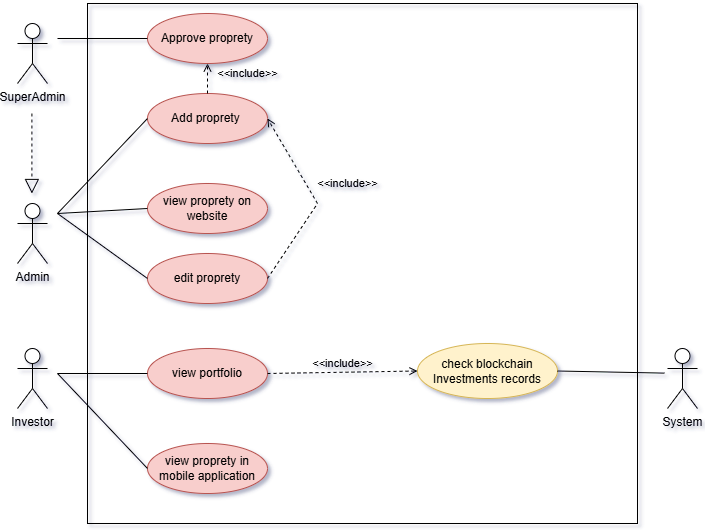
\includegraphics[width=0.8\textwidth]{images/property_portfolio_use_case.png}
    \caption{Property Management \& Investor Portfolio Use Case Diagram}
    \label{fig:property-portfolio-use-case}
\end{figure}

\subsubsection{Textual Use Case Descriptions}

\begin{table}[htbp]
    \centering
    \begin{tabular}{|p{3cm}|p{10cm}|}
        \hline
        \textbf{Use Case} & \textbf{Manage Property Listings} \\
        \hline
        \textbf{Actor} & Real Estate Agent, Administrator \\
        \hline
        \textbf{Precondition} & User is authenticated with appropriate permissions \\
        \hline
        \textbf{Main Scenario} & User creates, updates, or removes property listings \\
        \hline
        \textbf{Postcondition} & Property information is updated and available to investors \\
        \hline
    \end{tabular}
    \caption{Property Management Use Case Description}
    \label{tab:property-management-use-case}
\end{table}

\begin{table}[htbp]
    \centering
    \begin{tabular}{|p{3cm}|p{10cm}|}
        \hline
        \textbf{Use Case} & \textbf{Track Investment Portfolio} \\
        \hline
        \textbf{Actor} & Investor \\
        \hline
        \textbf{Precondition} & Investor has active investments in the platform \\
        \hline
        \textbf{Main Scenario} & Investor views portfolio performance and investment analytics \\
        \hline
        \textbf{Postcondition} & Comprehensive portfolio insights are displayed \\
        \hline
    \end{tabular}
    \caption{Investor Portfolio Use Case Description}
    \label{tab:investor-portfolio-use-case}
\end{table}

\subsection{Modeling}
\subsubsection{Class Diagram}
The property management and portfolio system follows object-oriented design principles with entities for properties, listings, investments, and analytics operations.

\begin{figure}[htbp]
    \centering
    % 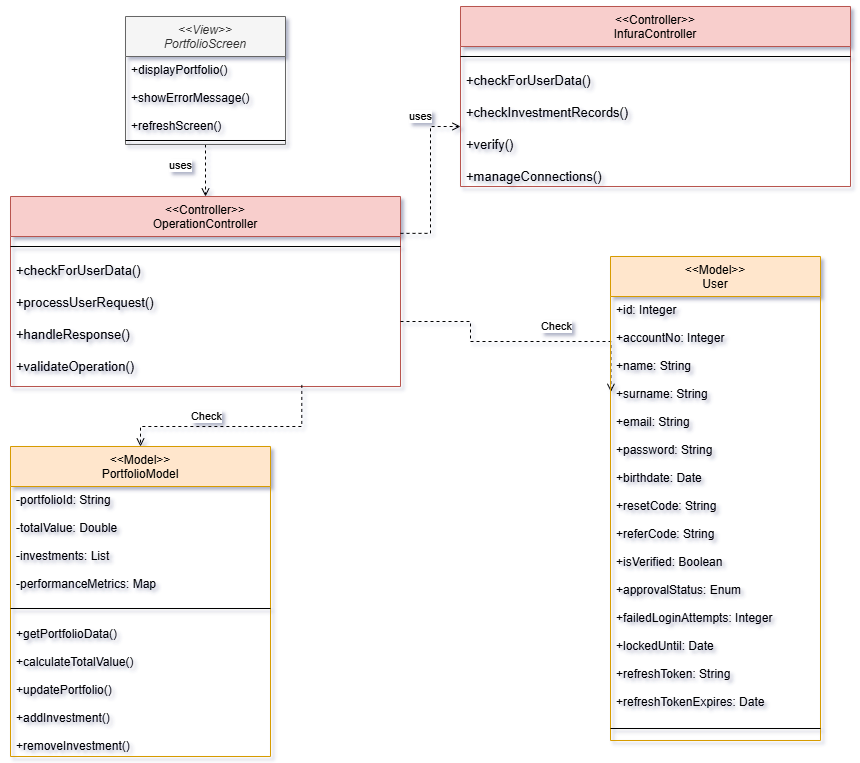
\includegraphics[width=0.9\textwidth]{images/property_portfolio_class_diagram.png}
    \caption{Property Management \& Investor Portfolio Class Diagram}
    \label{fig:property-portfolio-class}
\end{figure}

\subsubsection{Sequence Diagram}
The interaction sequence demonstrates the flow between user interface, backend services, and database operations for both property management and portfolio tracking operations.

\begin{figure}[htbp]
    \centering
    % 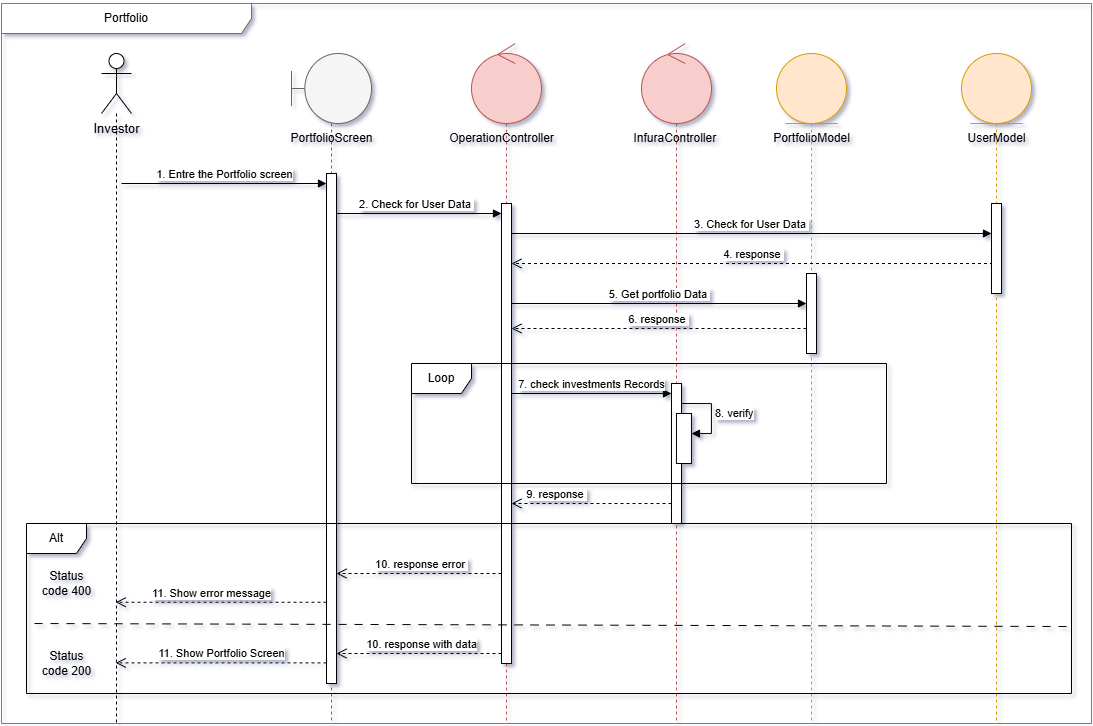
\includegraphics[width=1\textwidth]{images/property_portfolio_sequence.png}
    \caption{Property Management \& Investor Portfolio Sequence Diagram}
    \label{fig:property-portfolio-sequence}
\end{figure}

\subsection{Implementation}
\subsubsection{Property CRUD Operations}
The implementation includes comprehensive Create, Read, Update, and Delete operations for property management with advanced filtering and search capabilities. Property images and documents are managed through secure upload and storage systems with thumbnail generation and compression optimization.

\subsubsection{Portfolio Analytics Engine}
Advanced analytics engine calculating ROI, performance metrics, diversification indices, and risk assessments for investor portfolios. Real-time tracking of investment performance, rental income distribution, and capital appreciation across all investor holdings.

\subsubsection{Property Status Tracking}
Real-time tracking of property availability, investment status, and funding progress with automated status updates. Interactive charts and comprehensive reports providing insights into portfolio performance and investment trends.

\subsubsection{Reporting and Visualization}
Comprehensive dashboard combining property management tools with portfolio analytics, providing both agents and investors with the information they need to make informed decisions.

\subsection{Test}
\subsubsection{Functional Testing}
Comprehensive testing of all property management operations including creation, modification, and deletion workflows across different user roles. Analytics validation for portfolio calculations and performance metrics to ensure accuracy and reliability of financial data.

\subsubsection{Performance Testing}
Load testing for property search and filtering operations to ensure optimal performance with large property datasets. Extensive testing of portfolio dashboards and reporting features across web and mobile platforms.

\subsubsection{User Interface Testing}
End-to-end testing of the integrated property management and portfolio tracking interfaces to ensure seamless user experience across all functionality areas.

\subsection{Retrospective}

The Property Management \& Investor Portfolio sprint successfully delivered comprehensive property administration and investment tracking capabilities. Table \ref{tab:property-portfolio-retrospective} summarizes the key achievements and future improvements.

\begin{table}[htbp]
    \centering
    \begin{tabular}{|p{3cm}|p{10cm}|}
        \hline
        \textbf{Category} & \textbf{Details} \\
        \hline
        \textbf{What Went Well} & 
        \begin{itemize}
            \item Successfully implemented full CRUD operations for properties
            \item Portfolio analytics engine works accurately
            \item Integrated property and portfolio management interface
            \item Real-time investment tracking functions properly
            \item Interactive visualizations provide excellent insights
            \item Role-based access control functions across all features
        \end{itemize} \\
        \hline
        \textbf{Action Items} & 
        \begin{itemize}
            \item Implement advanced property comparison features
            \item Add predictive portfolio modeling capabilities
            \item Enhance property analytics and reporting integration
            \item Implement portfolio rebalancing recommendations
            \item Add bulk property import/export functionality
            \item Integrate with external financial planning tools
        \end{itemize} \\
        \hline
    \end{tabular}
    \caption{Property Management \& Investor Portfolio Sprint Retrospective Summary}
    \label{tab:property-portfolio-retrospective}
\end{table}

 